\chapter[Neutrino telescopes]{Breaking the cross section degeneracy: neutrino telescopes}
\label{ch:NT}

The presence of dark matter (DM) in the Solar neighbourhood provides us with the opportunity to directly detect its scattering in terrestrial detectors. As we have investigated in Chapter \ref{ch:Poly}, this may give us a handle on both the DM mass and speed distribution, providing we use a range of detector materials. However, the finite energy thresholds of direct detection experiments means that we cannot probe the entire range of DM speeds. With no sensitivity to low speed WIMPs, we also cannot know what fraction of WIMPs are probed by the experiments, resulting in a loss of sensitivity to the DM interaction cross section.

The local DM population may also scatter with nuclei in the Sun, becoming gravitationally captured if enough energy is lost in the interaction \cite{Press:1985,Silk:1985, Gaisser:1986, Srednicki:1987, Griest:1987}. These can then annihilate and produce neutrinos, which may be observed at neutrino telescope (NT) experiments such as IceCube. Importantly, capture occurs preferentially for WIMPs with low energy or, equivalently, low speed. Such a signal at an NT experiment would provide complementary sensitivity to the low speed WIMP population, hopefully breaking the degeneracy in the DM interaction cross section. 

In this chapter, we discuss the formalism for calculating the solar capture rate, as well as the processes of neutrino production, propagation and detection. We focus on calculating the event rate at the IceCube detector \cite{Aartsen:2013b}. We then test the polynomial $\ln f(v)$ parametrisation presented in Chapter \ref{ch:Poly} using both direct detection and IceCube mock data. In particular, we test the ability of these data sets to constrain the DM interaction cross sections and the DM mass, without making assumptions about the WIMP speed distribution. We note that due to the high abundance of spin-1/2 hydrogen in the Sun, we must consider both spin-independent (SI) and spin-dependent (SD) couplings in the analysis.


In Sec.~\ref{sec:NT:formalism}, we describe the IceCube event rate formalism. We then describe several particle physics and astrophysical benchmarks for the dark matter population in Sec.~\ref{sec:NT:experiments}, along with the experimental parameters used in the analysis. We explore the complementarity between NT and direct detection experiments in Sec.~\ref{sec:NT:complementarity}. In the remaining sections, we consider reconstructions of particle physics parameters first without IceCube data (Sec.~\ref{sec:NT:withoutIC}) and then with IceCube data (Sec.~\ref{sec:NT:withIC}), before discussing the prospects for reconstructing $f(v)$ itself (Sec.~\ref{sec:NT:speeddist}).

\section{Neutrino telescope formalism}
\label{sec:NT:formalism}
Calculation of the expected spectrum of neutrinos at an NT experiment can be broadly decomposed into 3 contributions. The first is the rate at which WIMPs scatter and are captured in the Sun. The second is the subsequent thermalisation of the solar WIMP population and their eventual annihilation into neutrinos. Third, we must model the detection of neutrinos at the IceCube detector. We now consider each of these in turn, focusing on the first, as this is where the WIMP cross sections and speed distribution enter into the calculation.

\subsection{Solar capture}

In calculating the solar capture rate, we follow closely the treatment of Gould \cite{Gould:1987,Gould:1992}. WIMPs are captured by the Sun when they elastically scatter off one of its constituent nuclei and end up with a speed lower than the solar escape velocity (which at the surface is equal to \(v_{\textrm{esc}}^\odot = 617.5 \kms\) \cite{Kaufmann:1991}). These WIMPs then enter bound orbits intersecting the Sun, ensuring further scatters with solar nuclei during subsequent passes. WIMPs may become unbound in subsequent scatters (this possibility will be discussed later) but typically lose energy until they collect and thermalise around the Sun's core.

\begin{figure}[h!]
    \centering
    \includegraphics[width=0.4\textwidth]{NT/Surface.pdf}
\caption[Geometry of WIMPs impinging on the Sun]{Illustration of the geometry of WIMPs impinging on the Sun}
\label{fig:NT:geometry}
\end{figure}

In order to calculate this `first-scatter' probability, we consider a spherical surface of radius $R$, large enough that the gravitational field at $R$ is negligible. This geometry is illustrated schematically in Fig.~\ref{fig:NT:geometry}. The number density of WIMPs with speed $v$ is $n_\chi f_1(v) \,\mathrm{d}v$. Because of the spherical symmetry of the problem, we can assume that the WIMP velocity distribution is isotropic without loss of generality. The fraction of WIMPs with direction $\cos \theta \rightarrow \cos \theta + \textrm{d} \cos \theta$ relative to the perpendicular direction is $\frac{1}{2} \textrm{d}\cos\theta$ (normalised over all values of $\cos \theta$). The WIMP speed perpendicular to the surface is given by $v \cos\theta$, meaning that the WIMP flux inward through the surface (per unit area) can be written:
\begin{equation}
\frac{n_\chi}{2} f_1(v) v \cos\theta \,\textrm{d}v \,\textrm{d}\cos\theta = \frac{n_\chi}{4} f_1(v) v \,\textrm{d}v \,\textrm{d}\cos^2\theta \,, \qquad \theta \in [0, \frac{\pi}{2}]\,.
\end{equation}
We change variables to angular momentum per unit mass, $ J = R v \sin\theta $, and integrate over all area elements on the surface of the shell to obtain the inward WIMP flux per unit time
\begin{equation}
4 \pi R^2 \frac{\rho_0}{m_\chi} \frac{1}{4}f_1(v) v \, \textrm{d}v \frac{\textrm{d}J^2}{R^2 v^2}.
\end{equation}

We now consider an inner shell of radius $r$ and thickness $dr$. If the escape velocity at the shell is $\vesc(r)$, then a WIMP with speed $v$ at infinity will have speed $w = \sqrt{v^2 + \vesc^2(r)}$ at this inner shell. The total time the WIMP spends in the shell is

\begin{equation}
\frac{\textrm{d}l}{w} = \frac{2}{w \cos \theta} \Theta(1 - \sin\theta) \, \textrm{d}r = \frac{2}{w}\left[ 1 - \left(\frac{J}{rw}\right)^2\right]^{-1/2} \Theta(rw - J) \, \textrm{d}r\,,
\end{equation}
where the Heaviside step function $\Theta$ appears because the WIMP crosses the shell either twice or not at all. If the rate at which a single WIMP travelling at velocity \(w\) is scattered down to a speed less than the escape speed \(\vesc\) is given by \(\Omega^{-}_{\vesc,i}(w)\), then we can write the WIMP capture rate per unit time as
\begin{align}
&2\pi \, \textrm{d}r \frac{\rho_0}{m_\chi}\frac{f_1(v)}{v}\,\textrm{d}v \frac{\ScatRate}{w}  \, \int_{0}^{(rw)^2} \left[ 1 - \left(\frac{J}{rw}\right)^2\right]^{-1/2} \, \textrm{d}(J^2) \nonumber\\&\qquad= 4 \pi r^2 \, \textrm{d}r \frac{\rho_0}{m_\chi} \frac{f_1(v)}{v}\, \textrm{d}v w \ScatRate\,.
\end{align}

The `first scatter' rate is then given by integrating over the radius of the Sun:
\begin{equation}
C_{\odot} = \frac{\rho_0}{m_\chi} \int_{0}^{R_{\odot}} \textrm{d}r \sum_i \dbd{C_i}{V} 4 \pi r^{2},
\end{equation}
where the capture rate per unit shell volume is
\begin{equation}
\label{eq:NT:dCdV}
\dbd{C_i}{V} = \int_{0}^{v_{\textrm{max}}} \textrm{d}v \frac{f_1(v)}{v} w \ScatRate\,.
\end{equation}
The index \(i\) labels the various nuclei in the Sun. The integration limit is
\begin{equation}
v_{\textrm{max}} = \frac{\sqrt{4m_\chi m_{N_i}}}{m_\chi - m_{N_i}}\vesc(r)\,.
\end{equation}
WIMPs above this speed cannot lose enough energy in a recoil to drop below the escape speed.

We now calculate the factor $\ScatRate$, which gives the rate at which a single WIMP travelling at velocity \(w\) is scattered down to a speed less than the escape speed \(\vesc\). This rate can be written as:
\begin{equation}
\ScatRate = \Phi_\chi N_T \sigma_{\vesc}\,
\end{equation}
where \(\Phi_\chi N_T\) is the WIMP flux multiplied by the number of target nuclei. For a single WIMP and a number density of nuclei \(n_N\), this becomes \( \Phi_\chi N_T = w n_N\). The cross-section for the process \(\sigma_{\vesc}\) is given by:
\begin{equation}
\label{eq:NT:sigma}
\sigma_{\vesc}  = \int_{E_{\vesc}}^{E_\textrm{max}} \dbd{\sigma}{E_R} \, \textrm{d}E_R\,
\end{equation}
where \(E_R = \Delta E\) is the energy lost by the scattering WIMP. The limits of integration run from the minimum energy loss required to reduce the WIMP speed below \vesc,
\begin{equation}
E_{\vesc} = \frac{m_\chi}{2}(w^2 - \vesc^2) = \frac{m_\chi}{2}v^2\,,
\end{equation}
to the maximum possible energy loss in the collision,
\begin{equation}
E_\textrm{max} = \frac{2 \mu_{\chi N}^2}{m_N} w^2\,.
\end{equation}

As in the direct detection case, we can decompose the differential cross section into SI and SD components. While all of the constituent elements of the Sun are sensitive to the SI interaction, only spin-1/2 Hydrogen is sensitive to SD scattering. The differential cross section is therefore given by

\begin{equation}
\dbd{\sigma}{E_R} = \frac{m_{N_i}}{2\mu_{\chi p}^2 v^2}
\begin{cases}
\sigmapsi + \sigmapsd & \textrm{ for } A = 1 \\
\sigmapsi A_i^2 F_i^2(E_R) & \textrm{ for } A > 1 \,.
\end{cases}
\end{equation}
No form factor is needed for Hydrogen ($A=1$), which consists of only a single nucleon. For the remaining nuclei, we approximate the form factor as \cite{Gould:1987}
\begin{equation}
F^2_i(E_R) = \exp(-E_R/E_i); \qquad E_i = \frac{3}{2m_{N_i} R_i^2}\,,
\end{equation}
where $R_i$ is the nuclear radius (see Sec.~\ref{sec:DD:nuclearunc}). These expressions allow Eq.~\ref{eq:NT:sigma} to be calculated analytically and introduce an error in the total capture rate of at most a few percent.
%%%%%%%%%%%%%%%%%%%%%%%%%%%%%
%%%%%%%%%%%%%%%%%%%%%%%%%%%%%\note{Might need some plots illustrating capture rates...}
%%%%%%%%%%%%%%%%%%%%%%%%%%%%%
In addition to the effects which have already been described, we can also consider a number of other factors which may impact the WIMP capture rate. The fact that nuclei in the Sun have a finite temperature has been neglected so far. However, detailed calculation \cite{Press:1985,Gould:1987} shows that this gives a correction to the capture rate of only around 1\% for WIMP masses above around 10 GeV. The gravitational influence of other bodies in the Solar system may also have an impact \cite{Gould:1991}. For example, Peter \cite{Peter:2009} found that WIMPs whose bound orbits reach out as far as Jupiter can be perturbed by the planet and become unbound. This leads to so-called \textit{Jupiter depletion} for WIMPs heavier than around 1 TeV. However, a recent study by Sivertsson and Edsj\"{o} \cite{Sivertsson:2012} showed using Liouville's theorem that such depletion processes must be accompanied by an inverse diffusion process. The net result is that for Solar capture we can treat the WIMP population as being free.



\subsection{Evolution of the WIMP population}

Once a WIMP has scattered to below the escape speed at a given solar position, it will be in a bound orbit and will enter the population of WIMPs captured by the Sun. Subsequent scatters with the nuclei in the Sun should lead to an approximately thermal distribution. There are then two processes which will tend to deplete this population: WIMP evaporation and annihilation.

Evaporation occurs when WIMPs scatter into the high speed tail of the thermal distribution, above the Solar escape velocity, and become unbound. It has been shown that for a WIMP mass of around 4 GeV, the evaporation timescale is approximately equal to the lifetime of the Sun ($\sim4.7$ billion years) \cite{Gould:1987b}. For WIMPs significantly heavier than this, the evaporation rate is negligible compared to the capture rate. For WIMPs lighter than this, the tail of the Maxwell-Boltzmann distribution lying above the escape velocity becomes significant and evaporation can no longer be neglected \cite{Krauss:1986,Busoni:2013b}. As we will see, the IceCube detector is sensitive to WIMPs with masses above around $m_\chi > 20 \textrm{ GeV} $, meaning that we can safely ignore the effects of evaporation.

The population of WIMPs will also undergo annihilation (either with their anti-particle partners or with themselves if they are Majorana particles). The evolution of the total number $N(t)$ of WIMPs in the Sun can then be written as \cite{Griest:1987}:

\begin{equation}
\dbd{N}{t} = C_c - \frac{1}{2}C_a N^2 - C_e N\,.
\end{equation}
The parameter $C_c$ is the total capture rate and the parameters $C_a$ and $C_e$ determine the annihilation and evaporation rates. As we have discussed, we can safely negelect evaporation, so we set $C_e$ to zero. The parameter $C_a$ and therefore the annihilation rate will depend on the velocity-averaged annihilation cross section $\langle \sigma v \rangle$ which is \textit{a priori} unknown. Over a long period of time, equilibrium between the capture and annihilation will be achieved and a steady state scenario for the WIMP population will be reached. This timescale is set by the equilibration time $\tau = 1/\sqrt{C_c C_a}$. If this is sufficiently short compared to the lifetime of the Sun, the WIMP population will currently be in equilibrium with the annihilation rate $\Gamma_a$ set by the capture rate as

\begin{equation}
\Gamma_a = \frac{1}{2}C_a\,.
\end{equation}

Crucially, in this case, the annihilation rate no longer depends on the unknown annihilation cross section, but is related only to the WIMP-nucleus scattering cross sections. We will assume in the rest of this chapter that the annihilation cross section is sufficiently high that the equilibrium assumption is valid.

Standard Model (SM) particles are produced in these annihilations, the majority of which cannot escape the Sun. However, some of these particles may decay to neutrinos or neutrinos may be produced directly in the WIMP annihilation. These neutrinos can escape the Sun and may be detected at NT experiments on Earth. It is important to account for the production and propagation of neutrinos in the dense medium of the Sun, as well as the propagation of these neutrinos from the Sun to the Earth \cite{Blennow:2008}. The spectrum of neutrinos reaching Earth can be written as

\begin{equation}
\dbd{N_\nu}{E_\nu} = \frac{\Gamma_a}{4\pi D^2}\sum_f B_f \dbd{N_\nu^f}{E_\nu}\,,
\end{equation}
where $D$ is the Earth-Sun distance, $\mathrm{d}N_\nu^f/\mathrm{d}E_\nu$ is the neutrino spectrum produced in the Sun for a particular final state $f$ and $B_f$ is the branching ratio into that final state. The branching ratios will depend on the specific form of the dark matter interactions with baryons. Typically, in order to set constraints on the WIMP interaction cross sections, we consider annihilation into only one channel at a time, assuming $B_f = 1$ for that particular channel during the analysis. Finally, the neutrino spectrum produced in the annihilation $\mathrm{d}N_\nu^f/\mathrm{d}E_\nu$ can be obtained using particle physics event generators (such as \textsc{Pythia} \cite{Sjostrand:1994}) and propagated to Earth using neutrino Monte Carlo simulations (such as WimpSim \cite{Blennow:2008}). We perform these calculations (and the capture rate calculation) using a modified version of the publicly available \textsc{DarkSUSY} package \cite{Gondolo:2004,DarkSUSYweb}.

%%%     arXiv:1402.4375 

%\note{Sub-section on propagation??? What should go in which section???}

\subsection{Detection}

Neutrinos which escape the Sun can be detected at terrestrial NT experiments \cite{Adrian-Martinez:2013,Aartsen:2013b}. We focus in this work on the IceCube experiment \cite{Abbasi:2009,Aartsen:2013b}, which can detect the \v{C}erenkov radiation produced by high energy particles traveling through ice. Muon neutrinos interact via charged-current interactions in the ice to produce relativistic muons. These in turn produce \v{C}erenkov light, which is collected by digital optical modules (DOMs) mounted on strings in the ice. The amount and pattern of lit DOMs allows the energy and direction of the incoming neutrino to be reconstructed.

In addition to the main IceCube array, a small region of the detector is instrumented with additional strings. This region has a DOM density roughly 5 times greater than the rest of the detector and is known as DeepCore \cite{Abbasi:2012}. The increased \v{C}erenkov light collection means that DeepCore lowers the threshold energy of the detector down to roughly 10 GeV. This gives the detector sensitivity to DM particles with mass down to around 20 GeV. Data from the 79-string IceCube experiment including DeepCore have been able to set upper limits of $\sigmapsi < 1.45 \times 10^{-43} \cmsq$ and $\sigmapsd < 1.34 \times 10^{-40}$ at the 90\% confidence level, for masses in the range 200-500 GeV and annihilation to $W^{+}W^{-}$ \cite{Aartsen:2013c}.


\section{Complementarity with direct detection}
\label{sec:NT:complementarity}
The complementarity between direct detection and NT data has been studied in the past \cite{Arina:2013}. In particular, the high abundance of hydrogen can help to constrain the spin-dependent cross section and, even in cases where no signal is observed at IceCube, limits from NT experiments can help to reduce the size of the allowed parameter space. Here, we explore further this complementarity by looking at the range of speeds which are probed by NT experiments.

As can be seen from Eq.~\ref{eq:NT:dCdV}, WIMPs with speeds from $v=0$ up to $v=v_\textrm{max}$ have the possibility of being captured by the Sun. In particular, with increasing WIMP speed the capture probability decreases, further suppressed by the loss of coherence in the SI case. As pointed out in Ref.~\cite{Choi:2014}, direct detection experiments probe a complementary range of the WIMP speed distribution, defined by the energy range of the WIMP search window. If the ranges of speeds probed by direct detection and NT experiments overlaps, this means that the entire WIMP speed distribution can be probed.

In Fig.~\ref{fig:NT:speedoverlap}, we show the WIMP speeds to which two experiments are sensitive as a function of WIMP mass. As a blue band, we show the region probed by a Xenon direction detection experiment. The lower and upper limits of the band are set by $v_\textrm{min}(\Emin)$ and $v_\textrm{min}(\Emax)$, where \Emin and \Emax define the extent of the WIMP signal window. In this chapter, we consider a window of $[5,45]$ keV. WIMPs with speeds above the blue band still contribute to the overall event rate (so there is still some sensitivity to them). However, there is no information on the \textit{shape} of the distribution at higher speeds, as we are not sensitive to the event spectrum above \Emax.


\begin{figure}[t]
  \centering
  \includegraphics[trim=0.8cm 0.9cm 0cm 0cm, clip,width=0.75\textwidth]{NT/SpeedOverlap.pdf}
  \caption[Speed sensitivity ranges of solar capture and direct detection experiments as a function of WIMP mass]{Sensitivity ranges of solar capture and direct detection experiments. We show as a blue band the range of speeds to which a Xenon detector is sensitive using an energy window of $[5,45]$ keV. The maximum speed to which solar WIMP capture is sensitive is shown as a solid (dashed) red line for SI (SD) interactions (see the text for more details).}
  \label{fig:NT:speedoverlap}
\end{figure}

Also shown in Fig.~\ref{fig:NT:speedoverlap} are the values of $v_\textrm{max}$ involved in the Solar capture rate for SI and SD interactions. In the SD case, the maximum speed is set by the hydrogen mass $m_H$:

\begin{equation}
v_{\textrm{max}} = \frac{\sqrt{4m_\chi m_H}}{m_\chi - m_H}\vesc\,.
\end{equation}
The escape speed \vesc depends on radius within the Sun so we use an average value, weighted by the hydrogen density as a function of radius. In the SI case, the situation is more complex, as more than one nucleus contributes to the capture rate. We therefore consider the average value of $v_\textrm{max}$ weighted by the mass fraction $f_i$ of each species

\begin{equation}
\langle v_{\textrm{max}} \rangle = \sum_i f_i \frac{\sqrt{4m_\chi m_{N_i}}}{m_\chi - m_{N_i}}\vesc\,,
\end{equation}
where again \vesc is evaluated at the average radius of each species $i$. This gives an indication of the typical value of $v_\textrm{max}$ experienced by WIMPs in the Sun.

In the SD case, the decreasing value of $v_\textrm{max}$ with $\mchi$ reflects the kinematics of the $\chi-H$ interaction. As the WIMP mass increases, scattering with hydrogen becomes less effecient at transferring energy. In the SI case, the value of $v_\textrm{max}$ is typically higher because the WIMP is closer in mass to the heavier nuclei in the Sun. However, there is still a significant SI interaction with hydrogen and the same fall off with $\mchi$ is observed as in the SD case. In addition, there are resonances in $v_\textrm{max}$, corresponding to perfect mass matching between the WIMP and one of the nuclei in the Sun. In these cases, energy transfer is highly efficient and WIMPs of any speed can scatter into bound orbits.

The key point of Fig.~\ref{fig:NT:speedoverlap} is that in both the SI and SD dominated cases, $v_\textrm{max}$ never falls below the lower limit of the blue band. This means that the combination of NT and direct detection data should provide sensitivity to the full range of WIMP speeds over a range of masses. The level of sensitivity may vary with WIMP speed, due for example to a falling capture contribution from higher speeds or form factor suppression in direct detection experiments. However, in principle, we can probe the full WIMP speed distribution and hopefully break the degeneracy in the cross section described in Chapter~\ref{ch:Poly}. The inclusion of data sets from additional direct detection experiments should only improve this sensitivity.

%\note{Need a linking paragraph here...}



\section{Benchmarks and experiments}
\label{sec:NT:experiments}
In order to test this complementarity and determine how well the WIMP parameters can be recovered, we generate mock data sets for a set of hypothetical direct detection experiments as well as for IceCube. In Table~\ref{tab:NT:experiments}, we show the parameters used in this chapter for three direct detection experiments chosen to mimic next-generation detectors currently in development. Each experiment is described by the range of nuclear recoil energies it is sensitive to and the total exposure (the product of the fiducial detector mass, the exposure time and the experimental and operating efficiencies). We also include a gaussian energy resolution of $\sigma_E = 1 \textrm{ keV}$ and a flat background rate of $10^{-7}$ events/kg/day/keV. This results in 1-2 background events in each detector. 

Compared to Chapter~\ref{ch:Poly}, we use a slightly lower threshold for the Xenon experiment. This is in light of the low threshold energy achieved by the LUX experiment \cite{Akerib:2014}. We use an exposure time $t_\textrm{exp} = 2 \textrm{ years}$ for all 3 experiments and a constant 50\% efficiency. The methods presented here would be used after a dark matter signal has been confirmed in multiple channels, once a sufficient number of events has been detected. We therefore choose not to model the energy resolution, background rates and efficiencies too closely on current experiments. Instead, we consider what may be possible with several somewhat-idealised future detectors.

For the spin-dependent scattering in Xenon and Germanium, we assume natural abundances of each of the isotopes and use the parametrisation of Cerdeno \etal \cite{Cerdeno:2012},

\begin{equation}
\label{eq:NT:SDparametrization}
S_{ij} = N ((1-\beta)\mathrm{e}^{-\alpha u} + \beta)\,,
\end{equation}
which is described in more detail in Sec.~\ref{sec:DD:nuclearunc}. The values we use 
for the parameters $(N, \alpha, \beta)$ for the $S_{00}$ spin structure functions are $(0.0595, 3.75, 0.0096)$ for Xe-129, 
$(0.035, 3.925, 0.12)$ for Xe-131 and $(0.195, 4.25, 0.07)$ for Ge-73. These 
were chosen to approximately reproduce the median values obtained from a range 
of spin structure function calculations \cite{Ressel:1993,Dimitrov:1995,Ressell:1997,Menendez:2012}. We focus in this work on understanding the impact of astrophysical uncertainties, so we keep the SD nuclear parameters fixed at these median values during the reconstructions.

We divide the energy range of each experiment into bins and generate Asimov data \cite{Cowan:2013} by setting the observed number of events in each bin equal to the expected number of events. While this cannot correspond to a physical realisation of data as the observed number of events will be non-integer, it allows us to disentangle the effects of Poisson fluctuations from the properties of the parametrisation under study.

\begin{table}[t]
  \setlength{\extrarowheight}{2pt}
  \begin{center}
%\begin{sideways}
	\begin{tabular}{c|m{1.2cm}m{2.2cm}m{2cm}m{2.1cm}}
        \hline\hline
	Experiment  & Target Mass, $A$ & Detector Mass (fid.), $m_\textrm{det}$/kg & Efficiency, $\epsilon$ & Energy Range/keV\\
	\hline
	Xenon  & 131  & 1000 & 0.5  & 5-45 \\
	Argon  & 40  & 1000 & 0.5  & 30-100  \\
        Germanium  & 73  & 300  & 0.5  & 10-100 \\
        \hline\hline
	\end{tabular}
%\end{sideways}
  \end{center}
\caption[Summary of parameters for mock direct detection experiments used in Chapter~\ref{ch:NT}]{Summary of parameters for mock direct detection experiments. All experiments have a constant energy resolution of $\sigma_E = 1 \textrm{ keV}$ and a flat background rate of $10^{-7}$ events/kg/day/keV. An exposure of $t_\textrm{exp} = 2 \textrm{ years}$ is used for all 3 experiments.}
\label{tab:NT:experiments}
\end{table}


To generate neutrino telescope data, we consider the IceCube 86-string configuration. We use an exposure time of 900 days (corresponding to five 180 day austral winter observing seasons, as in Ref.~\cite{Arina:2013}). We use an angular cut around the solar position $\phi_\textrm{cut} = 3\,^{\circ}$. This results in approximately 217 background events over the full exposure. As with the direct detection experiments, we set the observed number of events equal to the expected number of signal plus background events. We use only the observed number of events as data and not the energies of the individual events. Event-level likelihood methods have previously been developed \cite{Scott:2012} for use with IceCube 22-string data \cite{Abbasi:2009}. However, a similar analysis has not been performed for IceCube-86. In particular, the probability distributions for the number of lit digital optical modules (DOMs) as a function of neutrino energy are not yet available for IceCube-86. Nonetheless, using the number of observed events at IceCube is a first step towards using neutrino telescope data to help constrain the WIMP speed distribution.

\subsection{Benchmarks}
\label{sec:NT:benchmarks}
We use four benchmark models to generate mock data sets, which are summarised in Table~\ref{tab:NT:benchmarks}, along with the number of events expected for each model. In all cases, we use an SI WIMP proton cross section of $\sigmapsi = 10^{-45} \textrm{ cm}^2$ and SD cross-section of $\sigmapsd = 2 \times 10^{-40} \textrm{ cm}^2$, both of which are close to the current best exclusion limits \cite{Akerib:2014, Aprile:2013c}. For simplicity, we assume that the WIMP-proton and WIMP-neutron couplings are equal in both the SI and SD cases. We could allow the ratio of these couplings to vary as free parameters, but this would introduce additional degeneracies into the analysis. Here we focus on the degeneracy associated with the WIMP speed distribution.

Benchmark A represents an intermediate mass WIMP which annihilates to $W^{+}W^{-}$, which is similar to benchmark B used by Ref.~\cite{Arina:2013}. As we will see, even with this intermediate mass there is already a strong degeneracy in the reconstructed WIMP mass. We therefore choose not to consider a benchmark model with higher mass, which would result in an even poorer sensitivity to the reconstructed WIMP mass. We do, however, consider a lighter WIMP in benchmark C, which annihilates to $\nu_\mu \bar{\nu}_\mu$. The IceCube detector (with DeepCore) is sensitive to WIMPs with masses down to about 20 GeV. We therefore use a 30 GeV WIMP mass, as WIMPs much lighter than this cannot feasibly be detected by IceCube.

\begin{table}[pht!]
  \setlength{\extrarowheight}{3pt}
  \begin{center}
\begin{sideways}
	\begin{tabular}{c|ccm{2cm}|ccccccc}
        \hline\hline
	Benchmark & $m_\chi \textrm{ (GeV)}$ & Speed dist. & Ann. channel & $N_{\mathrm{Xe}}(SI)$ & $N_{\mathrm{Xe}}(SD)$  & $N_{\mathrm{Ar}}(SI)$ & $N_{\mathrm{Ar}}(SD)$ & $N_{\textrm{Ge}}(SI)$ & $N_{\textrm{Ge}}(SD)$ & $N_{\textrm{IC}}$ \\
	\hline
        A & 100 & SHM & $W^{+}W^{-}$ & 154.9 & 262.7 & 16.1 & 0 & 25.4 & 18.7 & 43.3\\
        B & 100 & SHM+DD & $W^{+}W^{-}$ & 167.1 & 283.9 & 16.2 & 0 & 25.7 & 18.9 & 242.9\\
        C & 30  & SHM & $\nu_\mu \bar{\nu}_\mu$ & 175.1 & 301.1 & 6.2 & 0 & 20.5 & 16.1 & 13.2\\
        D & 30  & SHM+DD & $\nu_\mu \bar{\nu}_\mu$ & 175.0 & 300.9 & 5.8 & 0 & 20.4 & 16.0 & 40.2\\
        \hline\hline
	\end{tabular}
\end{sideways}
  \end{center}
\caption[Summary of benchmarks used in Chapter~\ref{ch:NT}]{Summary of benchmarks. In all cases, we consider only isospin conserving interactions (i.e. $f_p = f_n$ and $a_p = a_n$). Also listed are the number of events foreseen in each detector. For direct detection targets we separate between recoils induced by SI and SD interactions.}
\label{tab:NT:benchmarks}
\end{table}

Benchmarks A and C assume an SHM speed distribution described by $v_\textrm{lag} = 230 \kms$ and $\sigma_v = 163 \kms$. Benchmarks B and D assume the same particle physics parameters as A and C respectively, but assuming an SHM distribution with a moderate dark disk overdensity (SHM+DD). We model the dark disk as contributing an additional 30\% dark matter density to the SHM, with parameters $v_\textrm{lag} = 50 \kms$ and $\sigma_v = 50 \kms$. As shown in Ref.~\cite{Choi:2013}, the capture rate in the Sun is not strongly dependent on variations in the shape of $f(v)$ (such as the differences between distribution functions extracted from different N-body simulations). However, significant enhancement of the capture rate can be achieved with the presence of a low speed dark disk, which we investigate using these two astrophysical benchmarks.


\subsection{Parameter sampling}
\label{sec:NT:sampling}
We perform parameter scans using a modified version of the publicly available \textsc{MultiNest 3.6} package \cite{Feroz:2007, Feroz:2008, Feroz:2014}. This allows us to map out the likelihood $\mathcal{L}(\theta)$ for the model parameters $\theta$.  We use $N_\textrm{live} = 20000$ live points in the scans and a tolerance of $10^{-4}$. We show in Table~\ref{tab:NT:priors} the priors on the various model parameters used in this work.

\begin{table}
  \setlength{\extrarowheight}{3pt}
  \begin{center}
%\begin{sideways}
	\begin{tabular}{ccc}
        \hline\hline
	Parameter & Prior range & Prior type \\
        \hline
        $m_\chi$ (GeV) & 10-1000 & log-flat \\
        $\sigma^p_{SI} \textrm{ (cm}^2\textrm{)}$ & $10^{-48} - 10^{-42}$ & log-flat \\
        $\sigma^p_{SD} \textrm{ (cm}^2\textrm{)}$ & $10^{-43} - 10^{-37}$ & log-flat \\
        Polynomial coefficients $\left\{a_k\right\}$ & $-20 - 20$ & linear-flat \\
        \hline\hline
        \end{tabular}
%\end{sideways}
  \end{center}
\label{tab:NT:priors}
\caption[Summary of \textsc{MultiNest} priors used in Chapter~\ref{ch:NT}]{Summary of \textsc{MultiNest} priors used in this chapter.}
\end{table}

In the polynomial $\ln f(v)$ parametrisation, we use 6 basis polynomials (5 free coefficients, with one fixed by normalisation). This is because, with the addition of SD interactions, the parameter space is significantly larger than in the SI-only case. As we will see, using 6 basis functions still allows a wide range of speed distributions to be explored and can provide a good fit to the data. With increasing numbers of events, it would be feasible to increase the number of basis functions and more precisely parametrise the form of the speed distribution.

The likelihood function we use for each experiment is:

\begin{equation}
\mathcal{L}(\theta) = \left(\prod_{i = 1, N_\textrm{bins}} \frac{(N_e^i)^{N_o^i}}{(N_o^i)!}e^{-N_e^i}\right)^{w}\,,
\end{equation}
where the signal region is divided into $N_\textrm{bins}$ bins with $N_e^i$ events expected and $N_o^i$ events observed in the $i$th bin. We weight the likelihood by a factor $w = N_\textrm{tot}/(N_\textrm{expt}N_\textrm{bins})$, where $N_\textrm{tot}$ is the total number of bins across all experiments. This means that the direct detection experiments (for which there are a large number of bins in energy) receive the same weight as the IceCube experiment (for which $N_\textrm{bins} = 1$). More details are given in Appendix~\ref{ch:ParamRecon}. The total likelihood is then the product over all experiments under consideration.

\section{Reconstructions without IceCube}
\label{sec:NT:withoutIC}

In Fig.~\ref{fig:NT:withoutIC}, we show the 2-dimensional profile likelihood plots for the parameters $(m_\chi, \sigmapsi)$, $(m_\chi, \sigmapsd)$ and $(\sigmapsi, \sigmapsd)$ reconstructed using the polynomial $\ln f(v)$ parametrisation. We use data from the three direct detection experiments described in Sec.~\ref{sec:NT:experiments} \textit{without} any additional information from IceCube. Each row corresponds to a different benchmark and the contours enclose the 68\% and 95\% confidence regions. The benchmark parameter values are shown as dashed red line, while the best fit is indicated as a green triangle. These results are distinct from the results of Chapter~\ref{ch:Poly} in that we are also including a contribution to the rate from spin-dependent interactions.

For Benchmark A (top row), there is a strong degeneracy in the WIMP mass. The benchmark value $m_\chi = 100 \textrm{ GeV}$ is larger than the target masses for Argon and Germanium, leading to a loss in sensitivity to the reconstructed WIMP mass. This is exacerbated by the degeneracy between $m_\chi$ and the shape of $f(v)$.  In spite of this, the best fit value is close to this benchmark value, indicating that the inclusion of SD scattering does not introduce any bias in the reconstruction of $m_\chi$. 

The inclusion of $\sigmapsd$ in the scan, however, does introduce an additional degeneracy in the overall event rate. At large masses the contours for \sigmapsd extend down to low values and we do not obtain a closed contour. The complementarity of different experiments has previously been studied in Ref.~\cite{Cerdeno:2013}. Because each target nucleus has a different response to SI and SD interactions, we should be able to determine the values of \sigmapsi and \sigmapsd separately. However, this depends on the uncertainties on the number of events at each experiment. For large $m_\chi$, the range of speeds probed by each experiment has less overlap (see e.g.~Fig.~\ref{fig:Speed:Access}). Because the experiments do not all probe the same range of speeds, there is more freedom, in varying $f(v)$, to reproduce the observed event numbers in each experiment. This means that a large $\sigmapsi$ and a small $\sigmapsd$ can account for the observed data. The same is not true for small values of $\sigmapsi$ and large values of $\sigmapsd$. This is because $\sigmapsi$ is constrained by the (small) number of events in the Argon experiment which couples only via SI interactions. A direct detection target such as Fluorine which is sensitive predominantly to SD scattering would allow the bounds on $\sigmapsd$ to be improved.

\todo{Should I include reconstructions with fixed f(v) - I could overlay them...}

\begin{figure}[pht!]
  \centering
  \includegraphics[trim=0.2cm 0.2cm 0.2cm 0.2cm, clip,width=0.32\textwidth]{NT/BenchmarkA_poly_noIC-mx_sigsi.pdf}
  \includegraphics[trim=0.2cm 0.2cm 0.2cm 0.2cm, clip,width=0.32\textwidth]{NT/BenchmarkA_poly_noIC-mx_sigsd.pdf}
  \includegraphics[trim=0.2cm 0.2cm 0.2cm 0.2cm, clip,width=0.32\textwidth]{NT/BenchmarkA_poly_noIC-sigsi_sigsd.pdf}

  \includegraphics[trim=0.2cm 0.2cm 0.2cm 0.2cm, clip,width=0.32\textwidth]{NT/BenchmarkB_poly_noIC-mx_sigsi.pdf}
  \includegraphics[trim=0.2cm 0.2cm 0.2cm 0.2cm, clip,width=0.32\textwidth]{NT/BenchmarkB_poly_noIC-mx_sigsd.pdf}
  \includegraphics[trim=0.2cm 0.2cm 0.2cm 0.2cm, clip,width=0.32\textwidth]{NT/BenchmarkB_poly_noIC-sigsi_sigsd.pdf}

  \includegraphics[trim=0.2cm 0.2cm 0.2cm 0.2cm, clip,width=0.32\textwidth]{NT/BenchmarkC_poly_noIC-mx_sigsi.pdf}
  \includegraphics[trim=0.2cm 0.2cm 0.2cm 0.2cm, clip,width=0.32\textwidth]{NT/BenchmarkC_poly_noIC-mx_sigsd.pdf}
  \includegraphics[trim=0.2cm 0.2cm 0.2cm 0.2cm, clip,width=0.32\textwidth]{NT/BenchmarkC_poly_noIC-sigsi_sigsd.pdf}

  \includegraphics[trim=0.2cm 0.2cm 0.2cm 0.2cm, clip,width=0.32\textwidth]{NT/BenchmarkD_poly_noIC-mx_sigsi.pdf}
  \includegraphics[trim=0.2cm 0.2cm 0.2cm 0.2cm, clip,width=0.32\textwidth]{NT/BenchmarkD_poly_noIC-mx_sigsd.pdf}
  \includegraphics[trim=0.2cm 0.2cm 0.2cm 0.2cm, clip,width=0.32\textwidth]{NT/BenchmarkD_poly_noIC-sigsi_sigsd.pdf}
\caption{2-dimensional profile likelihood for (\mchi, \sigmapsi) (left column), (\mchi, \sigmapsd) (central column) and (\sigmapsi, \sigmapsd) (right column), obtained using the polynomial $\ln f(v)$ parametrisation with direct detection data only. The shaded area gives the value of the profile likelihood, while the blue contours define the 68\% and 95\% confidence regions for the particle physics parameters. The 4 rows (from top to bottom) correspond to the 4 benchmakrs A, B, C and D. The dashed red lines show the position of the benchmark values from Tab. \ref{tab:NT:benchmarks} while the green triangle gives the best fit values.}
\label{fig:NT:withoutIC}
\end{figure}

The results for benchmark B (second row of Fig.~\ref{fig:NT:withoutIC}) share many features with those of benchmark A. This is because the majority of the dark disk population (which is present in benchmark B) lies at speeds below the energy thresholds of the experiments. However, a major difference is the extension of the contours up to large values of both $\sigmapsi$ and $\sigmapsd$. This is particularly evident in the top right corner of the right-most plot. This is an illustration of the problem described in both Chapter~\ref{ch:Speed} and Chapter~\ref{ch:Poly}: the shape of $f(v)$ is unconstrained at low $v$, which means that the fraction of WIMPs above the experimental thresholds is unconstrained. 

Why does this degeneracy not appear in benchmark A? This is because for a finite number $N$ of basis functions, the parametrisation we use for $f(v)$ cannot approximate all functional forms arbitrarily well. For large $m_\chi$, the lowest WIMP speed probed by the experiments is relatively small, with the Xenon experiment probing down to $v \approx 100 \kms$. Distributions which fit the data down to this low speed and then rise rapidly below it may not necessarily be well explored by the parametrisation. In benchmark B, the dark disk population causes a rise in $f(v)$ above $v \approx 100 \kms$, which leads to an excess in the data above the SHM-only case. For benchmark B, then, the parametrisation explores speed distributions which rise at low $v$ in order to reproduce the data. The unconstrained WIMP fraction below the threshold then leads to the observed cross section degeneracy.

We note that the cross section degeneracy is a real effect in the case of benchmark A, meaning that the reconstructed cross sections which appear in the top row of Fig.~\ref{fig:NT:withoutIC} must be taken as lower limits. The fact that this degeneracy does not appear in the profile likelihood is a consequence of the high WIMP mass and the finite number of basis functions used in the parametrisation. The degeneracy should become apparent with increasing $N$, but this would not improve the fit with the data, as it would simply explore a wider range of shapes for $f(v)$ below the experimental thresholds.

In benchmarks C and D (bottom two rows of Fig.~\ref{fig:NT:withoutIC}), the cross section degeneracy is pronounced, as the experiments now only probe down to $v\sim 200 \kms$ as a result of the lighter WIMP mass. The lighter WIMP mass also means that the rate is more sensitive to the reconstructed $m_\chi$ value. Thus, there is now an upper limit on $m_\chi$, though we can only constrain $m_\chi$ to within a factor of $\sim 4$ at the 68\% level. As in the case of heavier WIMP masses, \sigmapsd is not bounded from below due to the degeneracy between \sigmapsi and \sigmapsd.

\section{Reconstructions with IceCube}
\label{sec:NT:withIC}
In Fig.~\ref{fig:NT:withIC}, we show the profile likelihood reconstructed using the polynomial $\ln f(v)$ parametrisation (as in Fig.~\ref{fig:NT:withoutIC}) but now using both direct detection \textit{and} IceCube mock data. 

The results for benchmark A (top row) show that the best fit point is very close to the benchmark parameter values. One of the modes of the likelihood is peaked at the true WIMP mass and allows $m_\chi$ to be constrained to within a factor of 2 at the $1\sigma$ level. This is because the IceCube rate depends on $m_\chi$ in a different way to the direct detection experiments, leading to complementarity between the two experiments and allowing $m_\chi$ to be recovered more precisely. 

However, there is also a second mode in the likelihood, at large values of $m_\chi$ and low values of $\sigmapsd$. This is evident in the bottom right corner of the central panel on the top row. We have already discussed this scenario in the case of direct detection-only data. In addition, large WIMP masses result in higher energy neutrinos being produced in WIMP annihilations and therefore an increased number of events above the IceCube threshold \cite{Arina:2013}. This means that the lower value of \sigmapsd can also reproduce the observed IceCube data. Furthermore, distributions which rise rapidly at low $v$ can boost the capture rate further and therefore widen the allowed range of \sigmapsd to lower values.

The results for benchmark B (second row of Fig.~\ref{fig:NT:withIC}) are almost indistinguishable from the results of benchmark A. This indicates that the uncertainties in $f(v)$ are being well accounted for in each case. For benchmark B, the most striking difference when compared with the direct detection-only reconstructions is that the degeneracy of the cross sections up to large values has now been broken. Upper limits can now be placed on \sigmapsi and \sigmapsd at the 95\% level. Those points with large cross sections and a large WIMP population below the direct detection threshold would now overproduce events at IceCube, which is sensitive to this low speed WIMP population.

\begin{figure}[p!]
  \centering
  \includegraphics[trim=0.2cm 0.2cm 0.2cm 0.2cm, clip,width=0.32\textwidth]{NT/BenchmarkA_poly-mx_sigsi.pdf}
  \includegraphics[trim=0.2cm 0.2cm 0.2cm 0.2cm, clip,width=0.32\textwidth]{NT/BenchmarkA_poly-mx_sigsd.pdf}
  \includegraphics[trim=0.2cm 0.2cm 0.2cm 0.2cm, clip,width=0.32\textwidth]{NT/BenchmarkA_poly-sigsi_sigsd.pdf}

  \includegraphics[trim=0.2cm 0.2cm 0.2cm 0.2cm, clip,width=0.32\textwidth]{NT/BenchmarkB_poly-mx_sigsi.pdf}
  \includegraphics[trim=0.2cm 0.2cm 0.2cm 0.2cm, clip,width=0.32\textwidth]{NT/BenchmarkB_poly-mx_sigsd.pdf}
  \includegraphics[trim=0.2cm 0.2cm 0.2cm 0.2cm, clip,width=0.32\textwidth]{NT/BenchmarkB_poly-sigsi_sigsd.pdf}

  \includegraphics[trim=0.2cm 0.2cm 0.2cm 0.2cm, clip,width=0.32\textwidth]{NT/BenchmarkC_poly-mx_sigsi.pdf}
  \includegraphics[trim=0.2cm 0.2cm 0.2cm 0.2cm, clip,width=0.32\textwidth]{NT/BenchmarkC_poly-mx_sigsd.pdf}
  \includegraphics[trim=0.2cm 0.2cm 0.2cm 0.2cm, clip,width=0.32\textwidth]{NT/BenchmarkC_poly-sigsi_sigsd.pdf}

  \includegraphics[trim=0.2cm 0.2cm 0.2cm 0.2cm, clip,width=0.32\textwidth]{NT/BenchmarkD_poly-mx_sigsi.pdf}
  \includegraphics[trim=0.2cm 0.2cm 0.2cm 0.2cm, clip,width=0.32\textwidth]{NT/BenchmarkD_poly-mx_sigsd.pdf}
  \includegraphics[trim=0.2cm 0.2cm 0.2cm 0.2cm, clip,width=0.32\textwidth]{NT/BenchmarkD_poly-sigsi_sigsd.pdf}
\caption{As for Fig.~\ref{fig:NT:withoutIC} but including IceCube mock data. \todo{I might overlay the DD-only contours on here for comparison...}}
\label{fig:NT:withIC}
\end{figure}

For the light benchmarks (C and D, bottom two rows of Fig.~\ref{fig:NT:withIC}), the results are again largely indistinguishable, indicating good control over the astrophysical uncertainties. In both cases, the reconstruction of the mass is improved compared to the direct detection-only case, especially at low $m_\chi$. Due to the energy threshold at IceCube, the detector is only sensitive to the annihilation of WIMPs with masses above $\sim 25 \textrm{ GeV}$. WIMPs lighter than this cannot explain the number of excess events observed at IC. 

As in benchmarks A and B, we cannot place lower limits on \sigmapsd due to the remaining freedom in $f(v)$ at low speeds, which can boost $N_{IC}$. However, also as in the heavier benchmarks, the degeneracy in the cross sections up to high values is broken. We would like to determine the effect of IceCube data on the determination of the cross section. Due to the degeneracy between \sigmapsi and \sigmapsd, we will define an effective cross section $\sigma_\textrm{eff}$, which incorporates both cross sections and controls the overall event rate. Due to the different response of each detector to SI and SD couplings, we can define a different $\sigma_\textrm{eff}$ for each experiment (including IceCube). Here, we look at the effective cross section as seen by Germanium:

\begin{equation}
\label{eq:NT:sigeff}
\sigma_\textrm{eff} = \sum_{i} f_i A_i^2 \sigmapsi + f_{73} \frac{16\pi}{3} \frac{\sigmapsd}{2J+1} S_{00}(0)\,,
\end{equation}
where $f_i$ is the mass fraction of isotope $i$. In Fig.~\ref{fig:NT:sigeff}, we show the profile likelihood for $\sigma_\textrm{eff}$ with and without IceCube data (as solid and dashed lines respectively) for benchmark C. Without IceCube data, the profile likelihood of $\sigma_\textrm{eff}$ is almost entirely flat, with roughly 3 orders of magnitude uncertainty in the total WIMP interaction strength. Including IceCube data, the profile likelihood becomes sharply peaked, with the value of $\sigma_\textrm{eff}$ constrained to within a factor of 4 at the 68\% level. Clearly, the inclusion of IceCube data means that we can now reconstruct the value of the cross sections, rather than simply placing a lower limit.

\begin{figure}[!ht]
  \centering
  \includegraphics[width=0.75\textwidth]{NT/final018-sigeff.pdf}
\caption{Profile likelihood for the effective cross section $\sigma_\textrm{eff}$ of Germanium (defined in Eq.~\ref{eq:NT:sigeff}) with and without IceCube data for benchmark C. The vertical red dashed line corresponds to the benchmark value while the the vertical dotted black lines correspond to the limits of the 68\% and 95\% confidence intervals for the case \textit{with} IceCube data.}
\label{fig:NT:sigeff}
\end{figure}


\section{Reconstructing $f(v)$}
\label{sec:NT:speeddist}

As we are sensitive to the full range of WIMP speeds, we can now probe not only the shape of the speed distribution, as in Chapter~\ref{ch:Poly}, but the absolute value of $f(v)$. We show in Fig.~\ref{fig:NT:speedwithoutIC} the 68\% and 95\% confidence intervals (as grey bands) for the values of $f(v)$ using only direct detection data in benchmark B. These confidence intervals extend down to zero across almost the entire range of speeds, meaning that we cannot place any lower limit on $f(v)$. The degeneracy in the cross sections up to high values corresponds to a degeneracy in $f(v)$ down to low values. The results for the remaining benchmarks suffer from the same problem.

\begin{figure}[!ht]
  \centering
  \includegraphics[trim=0.5cm 0.5cm 0.5cm 0.5cm, clip,width=0.55\textwidth]{NT/BenchmarkB_poly_noIC-speed.pdf}
\caption{Reconstructed 68\% and 95\% confidence intervals (grey bands) for the directionally-averaged speed distribution $f(v)$ using only direct detection data. We show the SHM distribution (solid blue) and SHM+DD distributions (dashed green). Also shown in dashed red is the best fit form for $f(v)$. We note that for benchmark B, the true distribution is the SHM+DD.}
\label{fig:NT:speedwithoutIC}
\end{figure}

Including data from IceCube, the results are shown in Fig.~\ref{fig:NT:speedwithIC} for all 4 benchmarks. These result in significantly improved constraints on $f(v)$. For the case of A and B, the tightest constraints are obtained around $v \sim 100 \kms$. This is because for $m_\chi = 100 \textrm{ GeV}$ and the energy thresholds considered here, this is approximately the minimum speed probed by the experiments. This is where the most spectral information is available, as the rate decays with increasing energy. For the lower mass benchmarks (C and D), the best constraints are obtained for higher values of $v$, with a maximum sensitivity in the range $v=200-400 \kms$.

\begin{figure}[!pht]
  \centering
  \includegraphics[trim=0.5cm 0.5cm 0.5cm 0.5cm, clip,width=0.55\textwidth]{NT/BenchmarkA_poly-speed.pdf}
  \includegraphics[trim=0.5cm 0.5cm 0.5cm 0.5cm, clip,width=0.55\textwidth]{NT/BenchmarkB_poly-speed.pdf}
  \includegraphics[trim=0.5cm 0.5cm 0.5cm 0.5cm, clip,width=0.55\textwidth]{NT/BenchmarkC_poly-speed.pdf}
  \includegraphics[trim=0.5cm 0.5cm 0.5cm 0.5cm, clip,width=0.55\textwidth]{NT/BenchmarkD_poly-speed.pdf}
\caption{As Fig.~\ref{fig:NT:speedwithoutIC}, but for all 4 benchmarks, including data from both direct detection \textit{and} IceCube experiments. We show the SHM distribution (solid blue) and SHM+DD distributions (dashed green). Also shown in dashed red is the best fit form for $f(v)$. We note that for benchmarks A and C, the true distribution is the SHM, while for benchmarks B and D, the true distribution is the SHM+DD.}
\label{fig:NT:speedwithIC}
\end{figure}

The shape of $f(v)$ is less well constrained at low speeds because the IceCube data contains no spectral information. The capture rate is a single number, but depends on a combination of $m_\chi$, \sigmapsi, \sigmapsd and a series of integrals over $f(v)$. Thus, the precise shape of $f(v)$ at low speeds cannot be extracted, but the approximate magnitude of $f(v)$ can be inferred when IceCube and direct detection data are combined.

For benchmarks B and D, which have a SHM+DD distribution function, the best fit traces the benchmark distribution closely. In particular, the rise in the best fit $f(v)$ at low speeds indicates that we have achieved sensitivity to this low speed WIMP population. In the regions of maximum sensitivity, the value of $f(v)$ can be constrained to within a factor of around 4 at the 68\% level. We see that this uncertainty in the value of $f(v)$ is the source of the remaining uncertainty in the effective WIMP cross section $\sigma_\textrm{eff}$ described in the previous section, which can also be determined to within a factor of $\sim 4$. In spite of this remaining uncertainty, it may be possible to distinguish between different distribution functions. 

\section{Discussion}

We have demonstrated that for the benchmarks considered here, the WIMP mass can be better constrained with the inclusion of IceCube data and that the degeneracy in the cross sections up to high values (which is inherent in any astrophysics-independent analysis of data) can be broken.

The benchmarks we have considered in this chapter all result in a signal at IceCube. However, in benchmark C, the number of signal events is just 13, which is consistent with the observed background at just over $1\sigma$. Even with a signal of such low significance, we can still break the degeneracy between the cross section and $f(v)$. If we consider lighter WIMPs, which lie below the IceCube detection threshold, these would produce no events at IceCube regardless of the scattering cross sections and speed distribution. Thus, while we can use information from IceCube even with no significant signal, this would only give an improvement in constraints if the WIMP is heavy enough to potentially give a signal at IceCube.

Assuming that a signal is observed at IceCube, there is more information which can be extracted beyond simply the number of events. With the future release of information about energy reconstruction using the IceCube 86-string configuration, it should be possible to include spectral information in the analysis. This should significantly improve constraints on the mass and annihilation channel of the WIMPs, consequently improving constraints on the remaining parameters. However, because the capture rate depends only on an integral over the speed distribution, this additional spectral information will not allow us to significantly improve the shape reconstruction of $f(v)$ at low speeds.

We note that we have made several assumptions in this work. We have neglected uncertainties in spin-dependent form factors, which may result in wider uncertainties on the particle physics parameters. Using the parametrisation of Cerdeno \etal \cite{Cerdeno:2012} will allow us to take this into account, as well as to compare the relative importance of nuclear and astrophysical uncertainties. Further simplifications we have used include the assumptions of equilibrium between the capture and annihilation rates in the Sun, and the approximation that annihilations occur into a single channel.  These uncertainties could be relaxed and incorporated as additional fitting parameters. However, we have shown here what may be possible in an ideal case.

%\note{Higher order...}

The success of the method we have used here opens up the question of whether the inclusion of IceCube data can improve the performance of other speed distribution parametrisation methods. We could consider, for example, the case of the binned speed distribution studied by Peter \cite{Peter:2011} and studied in detail in Chapter~\ref{ch:Speed}. In that case, it was observed that the number and size of bins to which the experiments were sensitive depends in a specific way on the WIMP mass. The IceCube rate not only probes the low speed bins which are not accessible to direct detection experiments, but also depends on $m_\chi$ in a different way. This complementarity may therefore allow the bias caused by using the binned speed distribution to be reduced; lowering the WIMP mass will have a significant impact on the IceCube rate which may not result in a good fit to data. This perhaps opens up the possibility of using several different parametrisations to constrain the particle physics parameters as a consistency check.

Finally, the prospects for reconstructing the speed distribution seem good. In Fig.~\ref{fig:NT:speedwithIC}, for benchmark A, the SHM+DD distribution function falls outside the 68\% band. Similarly, for benchmark B, the SHM distribution lies outside the 68\% band at several different speeds. It is difficult to estimate the significance of rejecting these distributions. The bands in Fig.~\ref{fig:NT:speedwithIC} are calculated from the 1-dimensional profile likelihood separately at each value of $v$. However, the uncertainties at different values of $v$ are strongly correlated due to the normalisation of $f(v)$. This means that not all shapes falling within the 68\% band are consistent with the data at the 68\% level. However, if a speed distribution falls outside the 68\% band at some value of $v$, it can be rejected at at least the 68\% level. Further statistical analysis is required to determine the precise significance of the results of the $f(v)$ reconstructions.


Even if it is not possible reject these distributions with high significance using the data sets considered here, these results show that such a rejection should be possible with additional data. In Chapter~\ref{ch:Poly}, where only the \textit{shape} of $f(v)$ could be reconstructed, the SHM and SHM+DD distributions were almost indistinguishable. Including IceCube data we probe the low speed distribution, presenting the possibility of discriminating between the two astrophysical models and testing the existence of a dark disk in the Milky Way.


%%%%%%\note{Earth searches...?}

\section{Conclusions}

We have explored the possibility of combining neutrino telescope and direct detection data to probe a wider range of WIMP speeds. Neutrino telescopes, such as IceCube, are sensitive to the annihilations of WIMPs captured in the Sun. WIMPs with lower speeds are preferentially captured, meaning that IceCube probes a range of speeds complementary to those probed in direct detection experiments. In particular, this should allow the absolute value of $f(v)$ to be constrained, as well as breaking the degeneracy between the WIMP cross sections and the fraction of WIMPs above the detection threshold.

The inclusion of this data means that an upper limit can now be placed on the WIMP interaction cross sections, reducing the uncertainty on the total cross section by 2-3 orders of magnitude. However, the necessary inclusion of spin-dependent interactions opens up a new degeneracy direction. For the experiments considered here, it may not be possible to constrain the spin-dependent cross section from below. An increased exposure or a different choice of targets may improve this situation. However, this is not a problem associated with unknown astrophysics and has been previously observed even when no astrophysical uncertainties are taken into account \cite{Cerdeno:2013}.

Because we now probe the entire range of speeds of interest, we see improved constraints on the absolute value of $f(v)$. The maximum sensitivity is achieved near the threshold speeds of the direct detection experiments, where the most spectral information is available. This allows us to reconstruct $f(v)$ to within a factor of 4, opening up the possibility to distinguish the SHM from the SHM with an additional dark disk contribution, which was not previously feasible using direct detection-only data. 

Constraints on the WIMP mass are also improved, with the complementarity between IceCube and direct detection experiments allowing us to break the high mass degeneracy and begin to constrain $m_\chi$ to within a factor of 2 even for WIMP masses around 100 GeV. This is even possible with no significant signal observed at IceCube, although IceCube is insensitive to very low mass WIMPs and would therefore not improve constraints if the WIMP is lighter than around 20 GeV. The PINGU upgrade to IceCube \cite{Aartsen:2014} should lower the IceCube threshold and therefore allow a wider range of the parameter space to be explored and constrained.

We have demonstrated that combining direct detection data with IceCube, we can probe the entire range of WIMP speeds and reconstruct without bias the WIMP mass, SI and SD cross sections \textit{and} the values of the speed distribution itself, without making any astrophysical assumptions.



